% !Mode:: "TeX:UTF-8"
\chapter{车联网技术的网络资源优化理论基础}
\label{chap:figures}

插图主要涉及到:单个居中图形;两个并排图形;两个以上的并排或者堆叠的图形;图题;图形的引用;

\section{引言}\label{section2-1}
作为智能交通系统(ITS)最有前途的解决方案,车联网(IoV)有望满足快速增长的需求,如交通效率、驾驶体验和事故处理。然而,由于车辆密度和用户需求的快速增加,单小区网络的频谱效率较低\cite{TFL}。因此,异构车载网络的部署已成为一种趋势。

近年来,空地一体化作为提高无线通信质量的最可行的解决方案之一,引起了工业界和学术界的广泛关注。由于部署灵活、远程操作和中继能力,选择空中无人机来辅助地面网络\cite{ACO}。然而,当无人机加入异构场景时,空地综合通信网络将面临两大挑战。首先,当使用信道复用模式来提高频谱效率时,多用户干扰是一个棘手的问题。有效和稳健的通信在很大程度上受到多用户干扰的影响,特别是在不确定的信道环境中,因此实现有效的干扰管理是一个重大挑战\cite{ASO}。其次,空地集成异构车辆网络(AGHVN)是分层的,其中蜂窝用户(CUE)和车辆用户(VUE)分别充当领导者和追随者。然而,CUE和VUE是不同的利益相关者,他们为自己的利益而竞争。平衡各方利益是一项挑战。因此,空地一体化异构车载网络的广泛部署仍然带来紧迫的挑战。


\begin{comment}
\subsection{NOMA技术的理论基础}\label{section2-1-1}
大多数情况下,需要插入的图形是单个的时候可以使用如下环境:

\subsection{CR技术的理论基础}\label{section2-1-2}
其中的参数“[width=$\backslash$textwidth]”指定图形的宽度0.6倍页宽。最后的效果如图\ref{ysulogo}所示。
\begin{figure}[hptb!]
 \centering\small
 
\includegraphics[width=0.6\textwidth]{ysulogo}
 \Figcaption{单个居中图形}\label{ysulogo}
\end{figure}
\subsection{MEC技术的理论基础}\label{section2-1-3}

最终结果如图\ref{fig-dbfig}所示。
\begin{figure}[hptb!]
  \centering\small
  \begin{minipage}[t]{0.5\linewidth}
    \centering
    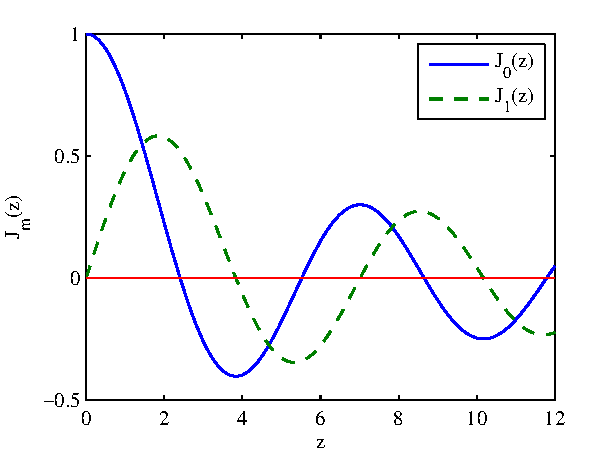
\includegraphics[width=\textwidth]{chp-2_bessel_j}
    (a) 子图a图题子图a图题子图a图题
  \end{minipage}%
  \begin{minipage}[t]{0.5\textwidth}
    \centering
    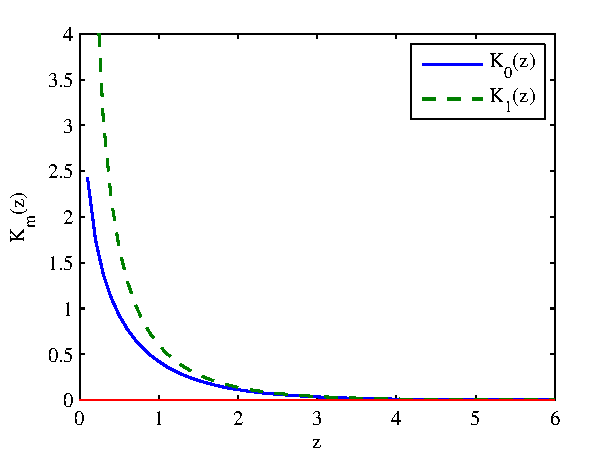
\includegraphics[width=\textwidth]{chp-2_bessel_k}
    (b) 子图b图题子图b图题子图b图题
  \end{minipage}
    \Figcaption{两个并排图形}\label{fig-dbfig}
 \end{figure}
\end{comment}

\section{问题构建}\label{section2-2}
\subsection{系统及信道模型}\label{section2-2-1}
我们考虑一种上行链路空地综合通信场景,其中大量的车辆到无人机(V2U)小区位于宏小区之下。
\subsection{博弈论问题}\label{section2-2-1}

啊 
\section{博弈问题求解}\label{section2-3}
\subsection{概率约束的转化}\label{section2-3-1}
\subsection{求解下层子问题}\label{section2-3-2}
\subsection{求解上层子问题}\label{section2-3-3}
\section{仿真验证及性能分析}\label{section2-4}

\section{本章小结}\label{section2-5}
在章节中,我们提出了一种基于鲁棒博弈的资源分配算法,以实现AGHVN中的有效信息传输。在新的优化方案中,关注用户之间的博弈关系,制定实时功率分配和定价策略,以最大限度地提高用户的利益。具体来说,为了保证系统的鲁棒性,引入概率约束来保证用户服务的可靠性和稳定性。由于通道不确定性的存在,概率形式是非凸的且难以处理的,在凸优化过程中采用了指数积分方法。根据仿真结果,功率和价格在几个步骤内收敛到最优值。我们还可以得出结论,Stackelberg对策优化方案表现出更好的鲁棒性。因此,在具有复杂多用户干扰和信道不确定性的空地一体化异构车载通信场景下,所提出的基于鲁棒博弈的资源分配算法是有效的。


\begin{comment}
\begin{verbatim}
\begin{figure}[hptb!]
  \centering\small
  \begin{minipage}[t]{0.5\linewidth}
    \centering
    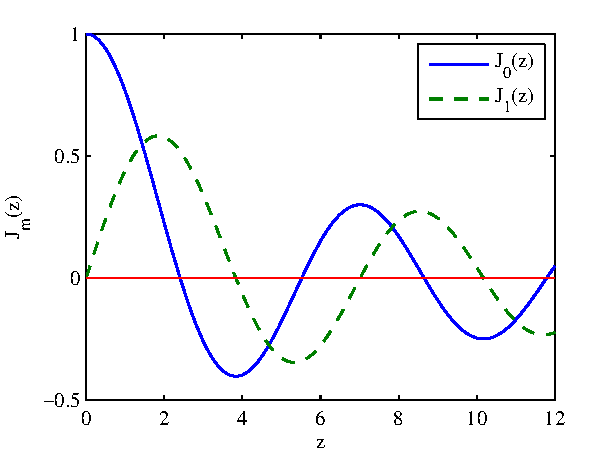
\includegraphics[width=\textwidth]{chp-2_bessel_j}
    (a) 子图a图题
  \end{minipage}%
  \begin{minipage}[t]{0.5\textwidth}
    \centering
    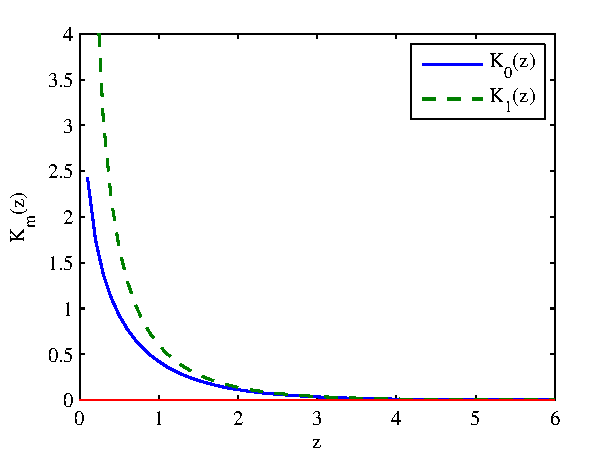
\includegraphics[width=\textwidth]{chp-2_bessel_k}
    (b) 子图b图题
  \end{minipage}  \\
  \begin{minipage}[t]{0.5\textwidth}
    \centering
    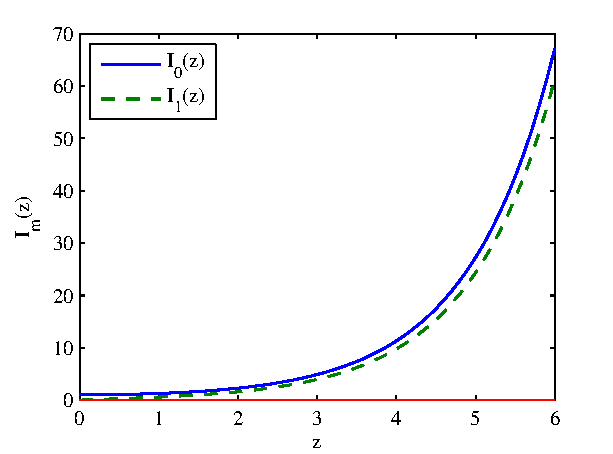
\includegraphics[width=\textwidth]{chp-2_bessel_i}
    (c) 子图c图题子图c图题子图c图题
  \end{minipage}%
  \begin{minipage}[t]{0.5\textwidth}
    \centering
    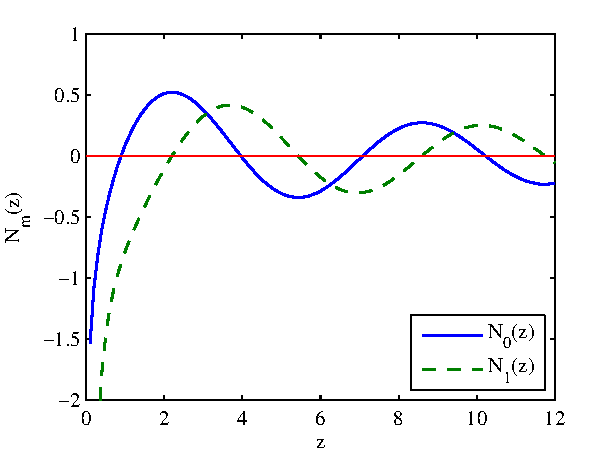
\includegraphics[width=\textwidth]{chp-2_bessel_n}
    (d) 子图d图题子图d图题子图d图题
  \end{minipage}
\Figcaption{贝塞尔函数}  \label{fig-bessel-function}
\end{figure}
\end{verbatim}
注意其中与一对并排图形不同的地方,加入了换行命令“$\backslash\backslash$”。
最终效果如图\ref{fig-bessel-function}所示。
\begin{figure}[hptb!]
  \centering\small
  \begin{minipage}[t]{0.5\linewidth}
    \centering
    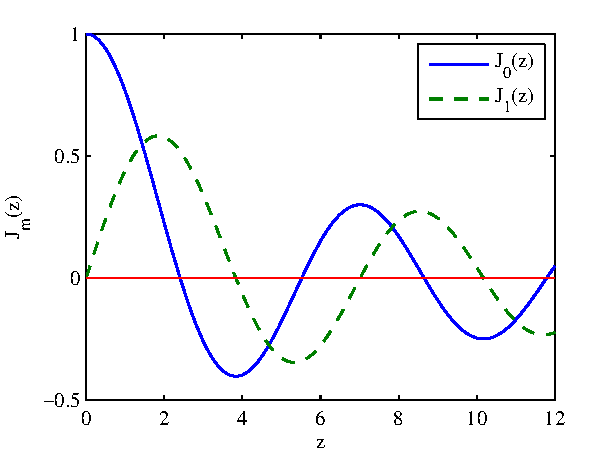
\includegraphics[width=\textwidth]{chp-2_bessel_j}
    (a) 子图a图题
  \end{minipage}%
  \begin{minipage}[t]{0.5\textwidth}
    \centering
    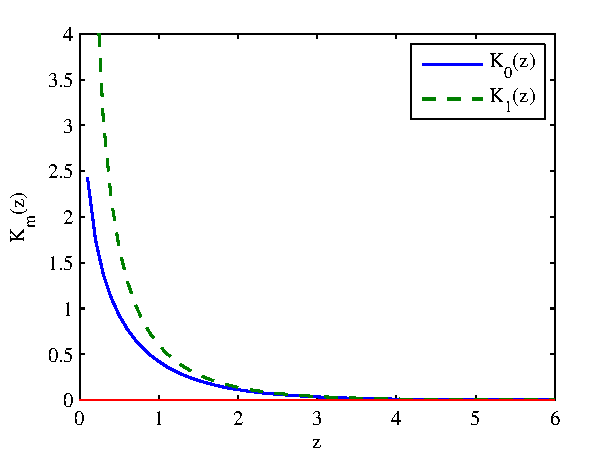
\includegraphics[width=\textwidth]{chp-2_bessel_k}
    (b) 子图b图题
  \end{minipage}  \\
  \begin{minipage}[t]{0.5\textwidth}
    \centering
    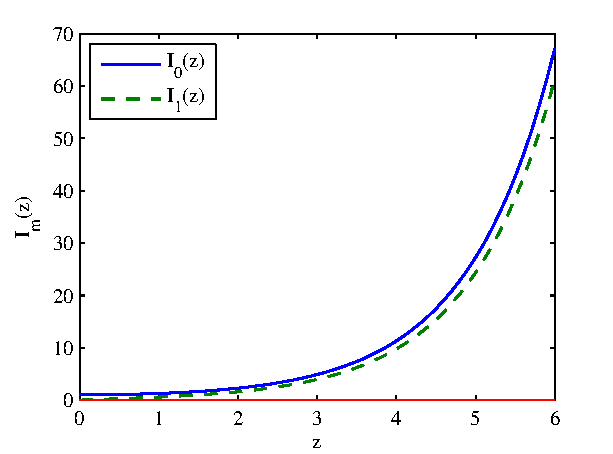
\includegraphics[width=\textwidth]{chp-2_bessel_i}
    (c) 子图c图题子图c图题子图c图题
  \end{minipage}%
  \begin{minipage}[t]{0.5\textwidth}
    \centering
    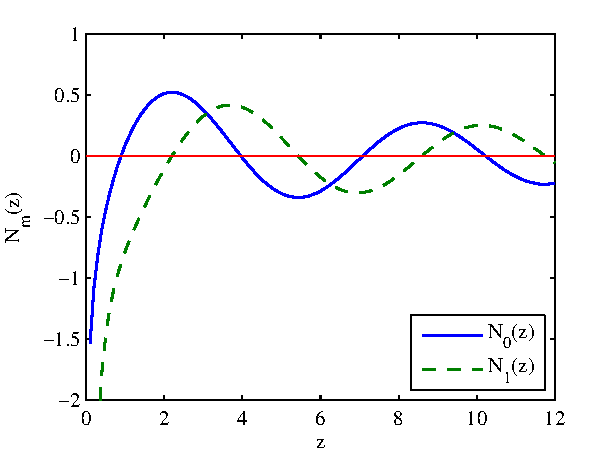
\includegraphics[width=\textwidth]{chp-2_bessel_n}
    (d) 子图d图题子图d图题子图d图题
  \end{minipage}
\Figcaption{贝塞尔函数}  \label{fig-bessel-function}
\end{figure}

其它类似的多个图形并排或者堆叠均可以灵活的运用minipage照猫画虎获得。

\section{图题}\label{section2-4}
其实上边的例子中已经包含了图题的引用命令\verb|\Figcaption|。
例如图\ref{fig-bessel-function}中:
\begin{verbatim}
    \Figcaption{贝塞尔函数}\label{fig-bessel-function}
\end{verbatim}
为当前的图形添加中文图题“贝塞尔函数”。同时添加标签“fig-bessel-function”。对图形的引用就是通过标签来实现的。

\section{图形的引用}\label{section2-5}
在已知图形的标签的基础之上,通过命令:
\begin{verbatim}
\ref{label}
\end{verbatim}
来引用标签为“label”的图形。\LaTeX 会自动将其替换为图形的编号。例如:
\begin{verbatim}
贝塞尔函数的图形如图\ref{fig-bessel-function}所示。
\end{verbatim}
的效果如下:\\
贝塞尔函数的图形如图\ref{fig-bessel-function}所示。


\section{本章小结}\label{section2-6}
注意!从第二章开始应有``本章小结",主要总结本章所做的主要研究工作,研究成果等内容!!!

%

\end{comment}

